% Provenance (never printed): see sources/outline_sources.md (Year 3:
% radial velocity, transits, imaging and microlensing; what has been
% found; atmospheres from transmission spectra).
% Brief: sources/book5/BRIEFS.md, ch. 28. Curves from figdata/bachelor-3/
% rv_transit.py (Keplerian radial-velocity curves, a limb-darkened transit
% light curve computed by numerical integration, point-lens microlensing)
% and exoplanet_archive.py (the NASA Exoplanet Archive's composite table of
% confirmed planets, fetched 2026-10-23, with the model mass--radius curves
% of Zeng et al.). Exercise and problem values in the Book 5 scratch
% calculator calc/ch28.py. Selene's Lamp and its planet are invented.
\chapter{Exoplaneten}\label{ch:b3:exoplanets}

In de herfst van 1994 maten twee astronomen de snelheden van 142
sterren vonden ze dat een van hen, 51~Pegasi, zich naar ons toe en van ons af bewoog,
met een periode van ongeveer vier dagen. De halve amplitude van de beweging was
\qty{59}{m.s^{-1}}, viermaal wat hun spectrograaf kon meten. De
begeleider die de ster rondtrok had minstens de helft van de massa van
Jupiter, op een baan van \qty{0.05}{au}, achtmaal dichter bij zijn ster
dan Mercurius bij de Zon staat. Geen theorie van planeetvorming had plaats voor
zo'n lichaam. De ontdekking, in oktober 1995 aangekondigd, opende een nieuw veld
van de sterrenkunde: drie decennia later zijn er meer dan zesduizend planeten rond
andere sterren bevestigd, enkele ervan zijn rechtstreeks waargenomen, en de
atmosfeer van sommige is geanalyseerd. Dit hoofdstuk laat zien hoe planeten die te zwak zijn
om te zien, worden gevonden, wat er gevonden is, en hoe hun atmosferen
worden afgelezen.
% ledger: nobel19:51peg, planet:Mercury.dist, data:b5-pscomp

\begin{recall}
Het dopplereffect, de radiële snelheid, spectroscopische dubbelsterren, de
wetten van Kepler, het tweelichamenprobleem en zijn zwaartepunt, de wet van Planck en de
schaalhoogte van een isotherme atmosfeer staan in de natuurkundeboeken. Een
exoplaneet en de bewoonbare zone van een ster staan in de schoolboeken.
De flux en de lichtkracht van een bron staan in Boek~3, in het
hoofdstuk over telescopen en fotometrie; de evenwichtstemperatuur, in het
hoofdstuk over vergelijkende planetologie. Planeetvorming en de sneeuwlijn
staan in Boek~4. Jeansontsnapping, \omterm{def:b3:planetary-atmospheres:hydrodynamic}{hydrodynamische ontsnapping} en de grenzen van
de bewoonbare zone staan in dit boek, in het hoofdstuk over planetaire
atmosferen.
\end{recall}

\section{De radialesnelheidsmethode}\label{sec:b3:exoplanets:rv}

Een planeet draait niet om zijn ster: beide draaien om hun gemeenschappelijk zwaartepunt.
De ster, veel zwaarder, beweegt op een eigen kleine baan, en zijn licht
wordt heen en weer dopplerverschoven met de periode van de planeet.

\begin{definition}[Radialesnelheidsmethode; minimale massa]\label{def:b3:exoplanets:rv}
De \emph{radialesnelheidsmethode}\index{radialesnelheidsmethode} detecteert een
planeet door de periodieke variatie van de radiële snelheid van zijn ster,
gemeten aan de dopplerverschuiving van de lijnen in het spectrum van de ster. Als
de inclinatie $i$ van de baan ten opzichte van het vlak van de hemel onbekend is, meet men
alleen het product $m_p\sin i$ van de massa van de planeet met de sinus van
de inclinatie, de \emph{minimale massa}\index{minimale massa} van de
planeet.
\end{definition}

\begin{theorem}[Halve amplitude van de radiële snelheid]\label{thm:b3:exoplanets:semi-amplitude}
Een ster met massa $M_\star$ en een planeet met massa $m_p$ op een cirkelbaan met
periode $P$, onder inclinatie $i$, geven de ster een radiële snelheid
$v_r(t) = \gamma + K\cos\bigl(2\pi(t - t_0)/P\bigr)$, met $\gamma$ de
snelheid van het zwaartepunt en de halve amplitude
\[
K = \left(\frac{2\pi G}{P}\right)^{1/3}
    \frac{m_p\sin i}{(M_\star + m_p)^{2/3}} .
\]
Bij een baan met excentriciteit $e$ is de kromme niet langer een sinusoïde,
$v_r = \gamma + K\bigl[\cos(\nu + \omega) + e\cos\omega\bigr]$, met $\nu$
de ware anomalie en $\omega$ het argument van het periastron, en $K$ wordt
gedeeld door $\sqrt{1 - e^2}$.
\end{theorem}

\begin{proof}
Voor de cirkelbaan: de afstand $a$ tussen de twee lichamen voldoet aan
de derde wet van Kepler, $a^3 = G(M_\star + m_p)P^2/4\pi^2$. De ster ligt op
de afstand $a_\star = a\,m_p/(M_\star + m_p)$ tot het zwaartepunt
en doorloopt zijn cirkel met de snelheid $v_\star = 2\pi a_\star/P$. Hieruit volgt
\[
v_\star = \frac{2\pi}{P}\,\frac{m_p}{M_\star + m_p}
          \left(\frac{G(M_\star + m_p)P^2}{4\pi^2}\right)^{1/3}
        = \left(\frac{2\pi G}{P}\right)^{1/3}\frac{m_p}{(M_\star + m_p)^{2/3}} .
\]
De zichtlijn maakt de hoek $\pi/2 - i$ met het vlak van de
baan, zodat alleen $v_\star\sin i$ van de snelheid van de ster langs de zichtlijn ligt, en
die component draait mee met de ster: $v_r - \gamma = v_\star\sin i\,
\cos\bigl(2\pi(t - t_0)/P\bigr)$. De excentrische vorm volgt uit de
keplerse ellips en wordt aangenomen.
\end{proof}

Omdat de planeet veel lichter is dan zijn ster, legt $K$ $m_p\sin i$ vast
zodra de periode is gemeten en de massa van de ster bekend is uit zijn
spectrum. Voor 51~Pegasi~b geldt $K = \qty{59}{m.s^{-1}}$ en $P = \qty{4.23}{d}$
rond een ster van één zonsmassa geven $m_p\sin i = 0.47$ Jupitermassa's.
Jupiter beweegt de Zon met \qty{12.5}{m.s^{-1}} over zijn baan van \num{4331}
dagen: een verre waarnemer zou de snelheid van de Zon zien schommelen met ongeveer
\qty{\pm 13}{m.s^{-1}} in twaalf jaar. De Aarde beweegt de Zon met
\qty{9}{cm.s^{-1}}. De spectrograaf die 51~Pegasi~b vond, haalde
\qty{13}{m.s^{-1}}; zijn opvolgers halen ongeveer \qty{1}{m.s^{-1}} (een
wandeltempo van \qty{3.5}{km/h}), en de nieuwste is gebouwd voor ongeveer
\qty{10}{cm.s^{-1}}, genoeg voor een planeet van aardmassa in de bewoonbare zone
van een ster met lage massa, waar de baan van de planeet kort is en de ster zelf weinig massa heeft.
De ster zelf legt een ondergrens: de pulsaties en vlekken van haar oppervlak,
die door haar rotatie worden meegevoerd, verschuiven ook haar lijnen, en het signaal van een planeet
moet daarvan worden onderscheiden.
% ledger: nobel19:51peg, nobel19:sun-jupiter, nobel19:migration, planet:Jupiter.mass, planet:Jupiter.Porb, planet:Jupiter.ecc, planet:Earth.mass, sun:mass, eso:espresso, const:G

\begin{omfigure}
\centering
\begin{tikzpicture}
\begin{axis}[width=0.86\linewidth, height=0.40\linewidth,
  xmin=0, xmax=2, ymin=-40, ymax=42,
  xlabel={orbitale fase (in perioden)}, ylabel={$v_r - \gamma$ (\unit{m.s^{-1}})},
  tick label style={font=\scriptsize}, label style={font=\small},
  legend style={font=\scriptsize, at={(0.5,-0.30)}, anchor=north, legend columns=2, draw=none, cells={anchor=west}, /tikz/every even column/.append style={column sep=1em}}]
\addplot[thin, black!40, forget plot] coordinates {(0,0) (2,0)};
\addplot[thick, omDef] table[x=phase, y=v_circ] {figdata/out/bachelor-3-rv_transit-rv.dat};
\addlegendentry{cirkelbaan}
\addplot[thick, dashed, red!70!black] table[x=phase, y=v_ecc] {figdata/out/bachelor-3-rv_transit-rv.dat};
\addlegendentry{$e = 0.3$, $\omega = \ang{60}$}
\draw[<->, thick] (axis cs:1.0,0) -- (axis cs:1.0,30);
\node[font=\scriptsize, anchor=east] at (axis cs:0.99,12) {$K$};
\end{axis}
\end{tikzpicture}
\par\smallskip{\small De radiële snelheid van een ster met één planeet, over
twee banen, voor een verzonnen planeet met $K = \qty{30}{m.s^{-1}}$ en een
periode van tien dagen. Op een cirkelbaan (doorgetrokken) is de kromme een sinusoïde
met halve amplitude $K$. Op een excentrische baan (gestreept) beweegt de ster
het snelst nabij het periastron, en de kromme wordt scheef: de uitersten zijn
$K(1 \pm e\cos\omega)$ en de piek-tot-piek-uitslag blijft
$2K$.}\label{fig:b3:exoplanets:rv}
\end{omfigure}

\section{Transits}\label{sec:b3:exoplanets:transits}

Als de baan bijna van opzij wordt gezien, schuift de planeet
eenmaal per omloop voor zijn ster en bedekt een klein deel van de schijf.

\begin{definition}[Transitmethode; transitdiepte; impactparameter]\label{def:b3:exoplanets:transit}
De \emph{transitmethode}\index{transitmethode} detecteert een planeet aan de hand van de
periodieke verzwakking van zijn ster wanneer de planeet over de stellaire schijf trekt. De
\emph{transitdiepte}\index{transitdiepte} $\delta$ is de fractionele afname
van de flux van de ster tijdens de transit. De
\emph{impactparameter}\index{impactparameter (transit)} $b = a\cos i/R_\star$ is de kleinste afstand
tussen de middelpunten van de planeet en de ster, gezien
aan de hemel, in eenheden van de stellaire straal $R_\star$, voor een baan
met straal $a$ en inclinatie $i$.
\end{definition}

\begin{proposition}[Transitdiepte]\label{prop:b3:exoplanets:depth}
Een donkere planeet met straal $R_p$ die volledig voor een ster met uniforme
helderheid staat, geeft de diepte $\delta = (R_p/R_\star)^2$.
\end{proposition}

\begin{proof}
De planeet bedekt het oppervlak $\pi R_p^2$ van een schijf met oppervlak $\pi R_\star^2$
die overal even helder is; de flux daalt evenredig.
\end{proof}

Jupiter die de Zon passeert, zou haar met \qty{1.06}{\percent} verzwakken, de Aarde
met \num{84} delen per miljoen: het eerste ligt binnen bereik van een kleine
telescoop, het tweede vraagt om een ruimtetelescoop die jaren lang duizenden
sterren meet. Een stellaire schijf is echter niet uniform.

\begin{definition}[Randverduistering]\label{def:b3:exoplanets:limb}
\emph{Randverduistering}\index{randverduistering} is de afname van de oppervlaktehelderheid
van een ster van het middelpunt van de schijf naar de rand, de limb.
Nabij de rand dringt de zichtlijn schuin de atmosfeer van de ster binnen
en bereikt een optische diepte van één in hogere, koelere lagen, die
minder uitstralen. Vaak wordt dit geschreven als een kwadratische wet in $\mu = \cos\theta =
\sqrt{1 - r^2}$, met $r$ de afstand tot het middelpunt van de schijf in
stralen van de ster: $I(\mu)/I(1) = 1 - u_1(1 - \mu) - u_2(1 - \mu)^2$.
\end{definition}

Een planeet nabij het middelpunt van een schijf met \omterm{def:b3:exoplanets:limb}{randverduistering} verbergt helderder licht
dan gemiddeld en verdiept de transit; nabij de rand verbergt hij minder. De
bodem van de lichtkromme is afgerond en de randen ervan worden zachter. De duur
van een transit draagt de geometrie in zich.

\begin{theorem}[Transitduur]\label{thm:b3:exoplanets:duration}
Voor een cirkelbaan met periode $P$, straal $a$ en inclinatie $i$, met
$p = R_p/R_\star$ en \omterm{def:b3:exoplanets:transit}{impactparameter} $b$, is de tijd van het eerste
contact tot het laatste:
\[
T_{14} = \frac{P}{\pi}\arcsin\!\left(\frac{R_\star}{a}\,
          \frac{\sqrt{(1 + p)^2 - b^2}}{\sin i}\right),
\]
en de tijd tussen het tweede en het derde contact, wanneer de planeet
volledig binnen de schijf staat, $T_{23}$, wordt gegeven door dezelfde formule
met $1 - p$ in plaats van $1 + p$.
\end{theorem}

\begin{proof}
Laat $\varphi = 2\pi t/P$ de baanfase zijn, geteld vanaf het midden van de transit.
Geprojecteerd op de hemel, met $x$ langs het pad van de planeet en $y$ dwars daarop,
ligt het middelpunt van de planeet op $x = a\sin\varphi$ en $y = a\cos i\cos\varphi$
vanaf het middelpunt van de ster. In eenheden van de stellaire straal is het gekwadrateerde afstand:
\[
z^2 = \left(\frac{a}{R_\star}\right)^2(\sin^2\varphi + \cos^2 i\cos^2\varphi)
    = \left(\frac{a}{R_\star}\right)^2\sin^2 i\,\sin^2\varphi + b^2 .
\]
De schijven raken elkaar van buitenaf wanneer $z = 1 + p$, bij
$\sin\varphi = \sqrt{(1 + p)^2 - b^2}\,R_\star/(a\sin i)$, symmetrisch
rond het midden van de transit. De transit duurt de fase $2\varphi$, dat is de
tijd $2\varphi P/2\pi = P\varphi/\pi$. Met $z = 1 - p$ raken de schijven
elkaar van binnenuit.
\end{proof}

Voor een wijde baan is de arcsinus gelijk aan zijn argument: $T_{14} \approx (P/\pi)
(R_\star/a)\sqrt{(1 + p)^2 - b^2}$. Een centrale transit duurt het langst; een
tangerende transit, met $b$ nabij $1 + p$, is kort en V-vormig. Door
$T_{14}$ en $T_{23}$ op een lichtkromme te meten, volgen $b$ en $a/R_\star$, en daarmee de
inclinatie: de transit legt de $\sin i$ vast die de radiële
snelheid onbekend laat.

\begin{omfigure}
\centering
\begin{tikzpicture}[scale=0.92]
\shade[inner color=yellow!25, outer color=orange!70] (0,0) circle (2);
\draw[orange!70!black] (0,0) circle (2);
\draw[dashed, black!60] (-3.2,-0.6) -- (3.2,-0.6);
\draw[->, black!60] (2.5,-0.6) -- (3.2,-0.6) node[right, font=\scriptsize] {pad};
\foreach \x in {-2.117, -1.697, 1.697, 2.117} {\fill[black] (\x,-0.6) circle (0.2);}
\node[font=\scriptsize] at (-2.117,-1.0) {1};
\node[font=\scriptsize] at (-1.697,-0.2) {2};
\node[font=\scriptsize] at (1.697,-0.2) {3};
\node[font=\scriptsize] at (2.117,-1.0) {4};
\fill[black] (0,0) circle (0.03);
\draw[<->, thick, omDef] (0,0) -- (0,-0.6) node[midway, left, font=\scriptsize] {$bR_\star$};
\draw[->] (0,0) -- (1.414,1.414) node[midway, above left, font=\scriptsize] {$R_\star$};
\end{tikzpicture}\hfill
\begin{tikzpicture}
\begin{axis}[width=0.52\linewidth, height=0.42\linewidth,
  xmin=-4, xmax=4, ymin=0.9855, ymax=1.0025,
  xlabel={tijd vanaf het midden van de transit (h)}, ylabel={relatieve flux},
  yticklabel style={/pgf/number format/fixed, /pgf/number format/precision=3},
  tick label style={font=\scriptsize}, label style={font=\small},
  legend style={font=\scriptsize, at={(0.5,-0.30)}, anchor=north, legend columns=1, draw=none, cells={anchor=west}, /tikz/every even column/.append style={column sep=1em}}]
\addplot[thick, omDef] table[x=t_h, y=flux_ld] {figdata/out/bachelor-3-rv_transit-transit.dat};
\addlegendentry{ster met randverduistering}
\addplot[thick, dashed, black!60] table[x=t_h, y=flux_uni] {figdata/out/bachelor-3-rv_transit-transit.dat};
\addlegendentry{uniforme ster}
\draw[densely dotted, black!50] (axis cs:-2.698,0.9855) -- (axis cs:-2.698,1.0025);
\node[font=\scriptsize, anchor=south] at (axis cs:-2.698,1.0005) {1};
\draw[densely dotted, black!50] (axis cs:-2.162,0.9855) -- (axis cs:-2.162,1.0025);
\node[font=\scriptsize, anchor=south] at (axis cs:-2.162,1.0005) {2};
\draw[densely dotted, black!50] (axis cs:2.162,0.9855) -- (axis cs:2.162,1.0025);
\node[font=\scriptsize, anchor=south] at (axis cs:2.162,1.0005) {3};
\draw[densely dotted, black!50] (axis cs:2.698,0.9855) -- (axis cs:2.698,1.0025);
\node[font=\scriptsize, anchor=south] at (axis cs:2.698,1.0005) {4};
\end{axis}
\end{tikzpicture}
\par\smallskip{\small Links: een planeet met $p = R_p/R_\star = 0.1$ kruist
de schijf van zijn ster bij de \omterm{def:b3:exoplanets:transit}{impactparameter} $b = 0.3$, bij de vier
contacten 1 tot en met 4; de schijf is donkerder naar de rand toe. Rechts: de lichtkromme
daarvan voor $a/R_\star = 15$ en een periode van tien dagen, berekend voor een
ster met de kwadratische randverduisteringscoëfficiënten $u_1 = 0.40$, $u_2 = 0.25$
(doorgetrokken) en voor een uniforme ster (gestreept, diepte precies $p^2 = 1\,\%$).
Tussen de contacten 2 en 3 is de lichtkromme met \omterm{def:b3:exoplanets:limb}{randverduistering} afgerond en dieper
dan $p^2$ nabij het midden van de transit.}\label{fig:b3:exoplanets:transit}
\end{omfigure}

\begin{proposition}[Transitkans]\label{prop:b3:exoplanets:probability}
Een planeet in een cirkelvormige baan met straal $a$, willekeurig georiënteerd,
transiteert zijn ster (met $b < 1$) met de kans $R_\star/a$.
\end{proposition}

\begin{proof}
Voor willekeurig georiënteerde banen is $\cos i$ uniform verdeeld tussen
0 en 1. De planeet transiteert wanneer $b = (a/R_\star)\cos i < 1$, dat wil zeggen
wanneer $\cos i < R_\star/a$, wat met kans $R_\star/a$ gebeurt.
\end{proof}

Een verre waarnemer zou de Aarde voor de Zon zien transiteren met een kans
van \qty{0.47}{\percent}, Jupiter met \qty{0.09}{\percent}. Een transitonderzoek
ziet slechts een klein deel van de planeten rond de sterren die het
waarneemt, en vooral de planeten die dicht bij hun ster staan.

Elke methode alleen laat iets weg. De radiële snelheid geeft
$m_p\sin i$; de transit geeft $R_p/R_\star$ en $i$. Samen geven ze
de ware massa en de straal, en daarmee de gemiddelde dichtheid
$\bar\rho = 3m_p/4\pi R_p^3$, de eerste aanwijzing over waaruit een planeet bestaat.
De eerste transits, begin 2000 gerapporteerd, betroffen een planeet die
al bekend was uit de snelheid van haar ster, HD~209458~b. Haar twee transits
toonden de \omterm{def:b3:exoplanets:limb}{randverduistering} van de ster en gaven een straal van 1.27 Jupiterstralen bij een inclinatie van
\ang{87.1}. Met de massa en straal uit het archief bedraagt haar gemiddelde dichtheid
\qty{0.34}{g.cm^{-3}}, een derde van die van water: een gasreus die opgeblazen is door de
warmte van haar ster.
% ledger: planet:Jupiter.diameter, planet:Earth.diameter, sun:R, const:au, planet:Jupiter.dist, charbonneau00:hd209458, nobel19:transits, data:b5-pscomp

Een transiterende planeet houdt de tijd goed bij. Trekt een tweede planeet eraan, dan
komen haar transits vroeg of laat, in een patroon dat zich herhaalt met
de gravitationele wisselwerking.

\begin{definition}[Variatie in transittijden]\label{def:b3:exoplanets:ttv}
Een \emph{variatie in transittijden}\index{variatie in transittijden} is de
afwijking van de tijdstippen van de transits van een planeet ten opzichte van een strikt periodieke
reeks, veroorzaakt door de gravitationele aantrekking van een ander lichaam in het
systeem; daarmee kunnen planeten worden onthuld en gewogen
die zelf niet transiteren.
\end{definition}

Een helling in een lichtkromme is niet altijd een planeet. Een verduisterend
sterpaar dat slechts schampt, of een zwak verduisterend sterpaar achter het doelwit waarvan het
licht wordt verdund door dat van het doelwit, kan een transit nabootsen. Een kandidaat wordt
een planeet wanneer zijn massa wordt gemeten, met de radiële snelheid of met
variaties in de transittijden, of wanneer elke andere verklaring is uitgesloten.

\section{Beeldvorming en microlensing}\label{sec:b3:exoplanets:imaging}

\begin{definition}[Directe beeldvorming; coronagraaf]\label{def:b3:exoplanets:imaging}
\emph{Directe beeldvorming}\index{directe beeldvorming} detecteert een planeet aan zijn eigen
licht, teruggekaatst of uitgezonden, dat op de hemel gescheiden is van het licht van
zijn ster. Een \emph{coronagraaf}\index{coronagraaf} is een instrument dat het
licht van de ster in het brandpunt van de telescoop blokkeert, met een masker of door de
interferentie van het licht, zodat zwakke bronnen dicht bij de ster
zichtbaar worden.
\end{definition}

De moeilijkheid is tweeledig. Een baan van \qty{1}{au}, gezien vanaf \qty{10}{pc},
beslaat slechts \ang{;;0.1}, en de planeet is vele ordes van grootte zwakker
dan haar ster. Jonge reuzenplaneten zijn de gemakkelijkste doelen: nog heet van
hun vorming gloeien ze in het infrarood, waar het contrast met hun
ster het kleinst is. In 2008 toonden beelden van twee grote telescopen drie
planeten rond de ster HR~8799, op projectieafstanden van 24, 38 en
\qty{68}{au}, die van jaar tot jaar tegen de klok in bewogen; hun
lage lichtkracht en de ouderdom van het systeem geven ze een massa van 5 tot
13 Jupitermassa's. De planeet op de foto hieronder ligt op \ang{;;0.82} van zijn
ster; de coronagrafen van de ruimtetelescoop bereiken een contrast van
\num{1e-5} bij \ang{;;1} en \qty{4.4}{\micro m}.
% ledger: iau:parsec, const:au, marois08:hr8799, carter23:hip65426

\begin{omfigure}
\centering
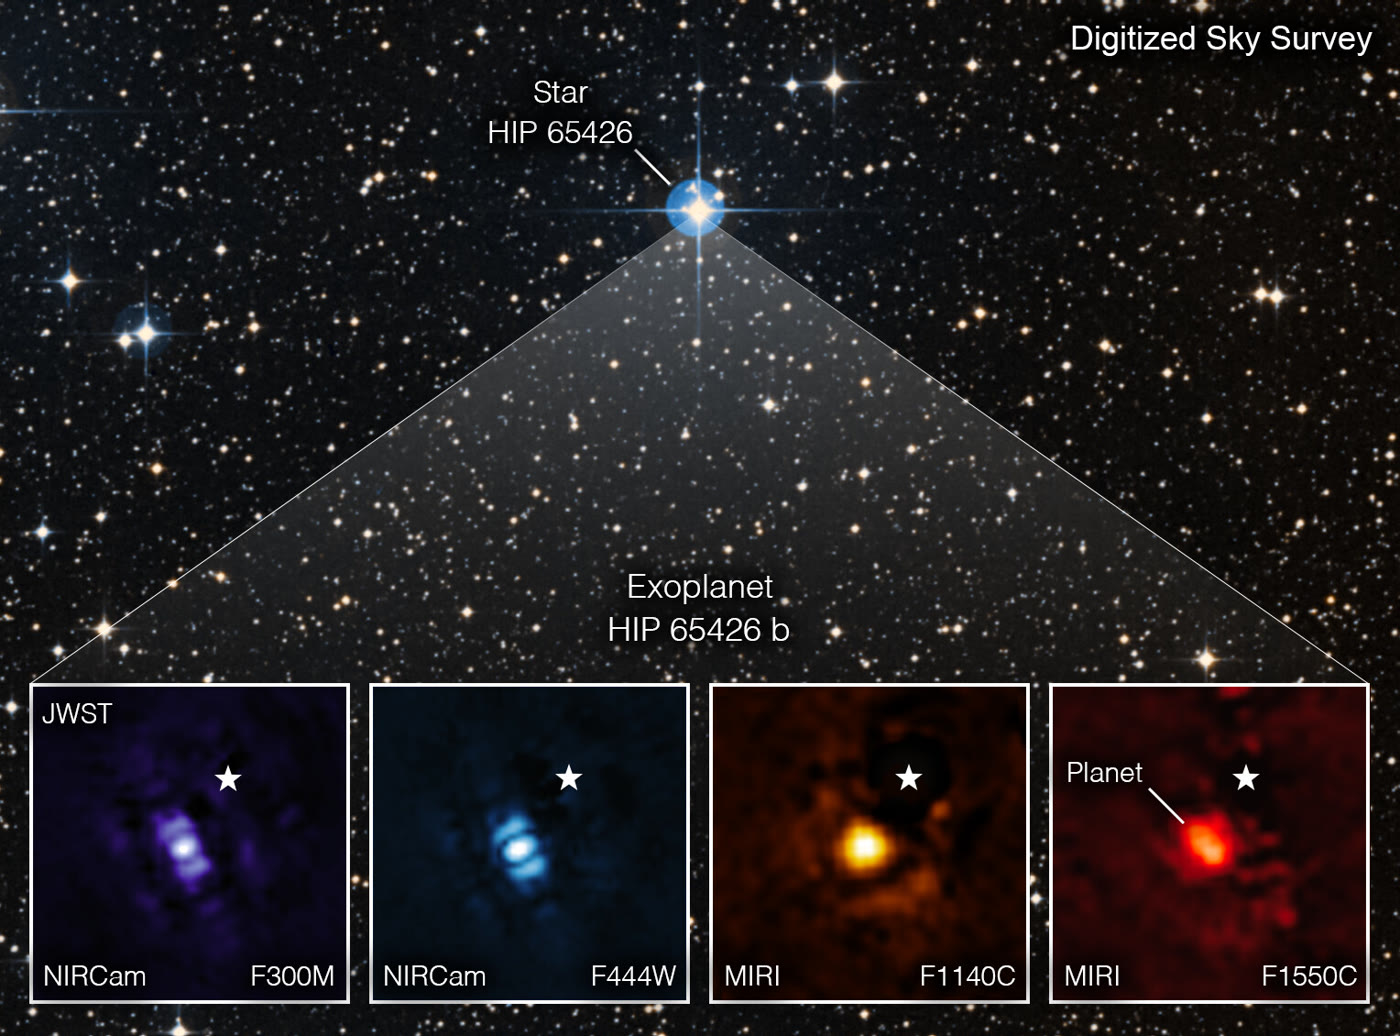
\includegraphics[width=0.86\linewidth]{images/book5/b3-hip65426b.jpg}
\par\smallskip{\small De eerste exoplaneet die door de James Webb Space
Telescope is afgebeeld, HIP~65426~b, in vier infraroodfilters (onder; boven het
beeldveld van de ster uit een vanaf de grond uitgevoerde hemelsurvey); het licht van
de ster, op de plek van het sterrensymbool, wordt door de
coronagrafen geblokkeerd. De planeet is een jonge gasreus van ongeveer 6 tot 8
Jupitermassa's, ruwweg 15 tot 20 miljoen jaar oud, ongeveer honderd keer
verder van haar ster af dan de Aarde van de Zon. Beeld NASA/ESA/CSA,
A~Carter (UCSC), het ERS~1386-team, en A.~Pagan (STScI), CC
BY~4.0.}\label{fig:b3:exoplanets:hip65426}
\end{omfigure}
% ledger: photo:b3-hip65426b

Een vierde methode gebruikt de zwaartekracht als lens. Wanneer een ster bijna precies
voor een verder weggelegen ster langs schuift, buigt zijn zwaartekracht het licht van de
achtergrondster en maakt die gedurende enkele weken helderder; een planeet van de
lensende ster voegt een korte piek toe.

\begin{definition}[Gravitationele microlensing; Einstein-straal]\label{def:b3:exoplanets:microlensing}
\emph{Gravitationele microlensing}\index{gravitationele microlensing} is het
tijdelijk helderder worden van een achtergrondster wanneer een voorgrondster, de
lens, dicht langs de zichtlijn passeert; de beelden die ze vormt liggen te dicht
bij elkaar om te kunnen worden onderscheiden. De \emph{Einstein-straal}\index{Einstein-straal}
is de hoekstraal $\theta_\mathrm E$ van de ring waarin een puntlens
met massa $M$ op afstand $D_L$ een bron op afstand $D_S$ precies erachter
tot een ring zou vervormen:
\[
\theta_\mathrm E = \sqrt{\frac{4GM}{c^2}\,\frac{D_S - D_L}{D_L D_S}} .
\]
\end{definition}

\begin{proposition}[Vergroting door een puntlens]\label{prop:b3:exoplanets:magnification}
Een bron op hoekafstand $u\,\theta_\mathrm E$ van een puntlens
wordt met de factor helderder:
\[
A(u) = \frac{u^2 + 2}{u\sqrt{u^2 + 4}} .
\]
\end{proposition}

\admitted

Beide resultaten volgen uit de buiging van licht door een massa in de algemene
relativiteitstheorie. Voor een lens met een halve zonsmassa, halverwege een bron
die \qty{8}{kpc} ver weg staat, geldt $\theta_\mathrm E = \qty{0.71}{mas}$, en
heeft de Einsteinring, op de afstand van de lens, een straal van \qty{2.9}{au}. Bij
$u = 1$ is de bron 1.34 keer helderder, bij $u = 0.1$ tien keer. Een
planeet nabij de Einsteinring van zijn ster voegt een korte afwijking toe aan de
lichtcurve. \omterm{def:b3:exoplanets:microlensing}{Gravitationele microlensing} vindt zo planeten op enkele astronomische
eenheden van hun ster, koude planeten die de \omterm{def:b3:exoplanets:transit}{transitmethode} en de \omterm{def:b3:exoplanets:rv}{radialesnelheidsmethode} missen,
maar elke gebeurtenis gebeurt eenmalig en wordt nooit herhaald. Bij een gebeurtenis uit 2003,
gepubliceerd het jaar erna, duurde een afwijking van ongeveer zeven dagen en werd
alleen verklaard door een begeleider van $\num{0.0039}$ keer de massa van de
lens: een planeet van ongeveer 1.5 Jupitermassa op ongeveer \qty{3}{au} van
zijn ster.
% ledger: const:G, const:c, sun:mass, iau:parsec, const:au, bond04:ogle235

\begin{omfigure}
\centering
\begin{tikzpicture}[scale=0.95]
\fill (0,0) circle (0.06) node[below=2pt, font=\scriptsize] {bron};
\fill[omDef] (3.2,0) circle (0.09); \node[font=\scriptsize, omDef] at (3.2,-1.15) {lens};
\draw[omDef] (3.2,0) ellipse (0.12 and 0.9);
\fill (6.4,0) circle (0.06) node[below=2pt, font=\scriptsize] {waarnemer};
\draw[thick, orange!80!black] (0,0) -- (3.2,0.9) -- (6.4,0);
\draw[thick, orange!80!black] (0,0) -- (3.2,-0.9) -- (6.4,0);
\draw[densely dashed, black!50] (6.4,0) -- (0,1.8) node[left, font=\scriptsize] {beeld};
\draw[densely dotted, black!50] (0,0) -- (6.4,0);
\draw[<->] (3.55,0) -- (3.55,0.9) node[midway, right, font=\scriptsize] {$R_\mathrm E$};
\draw[<->, black!60] (0,-1.5) -- (3.2,-1.5) node[midway, below, font=\scriptsize] {$D_S - D_L$};
\draw[<->, black!60] (3.2,-1.5) -- (6.4,-1.5) node[midway, below, font=\scriptsize] {$D_L$};
\end{tikzpicture}\hfill
\begin{tikzpicture}
\begin{axis}[width=0.48\linewidth, height=0.42\linewidth,
  xmin=-3, xmax=3, ymin=0.8, ymax=12, ymode=log,
  ytick={1,2,5,10}, yticklabels={1,2,5,10},
  xlabel={tijd ($t_\mathrm E$)}, ylabel={vergroting $A$},
  tick label style={font=\scriptsize}, label style={font=\small},
  legend style={font=\scriptsize, at={(0.5,-0.30)}, anchor=north, legend columns=3, draw=none, cells={anchor=west}, /tikz/every even column/.append style={column sep=1em}}]
\addplot[thick, omDef] table[x=t_tE, y=A01] {figdata/out/bachelor-3-rv_transit-lens.dat};
\addlegendentry{$u_0 = 0.1$}
\addplot[thick, dashed, red!70!black] table[x=t_tE, y=A03] {figdata/out/bachelor-3-rv_transit-lens.dat};
\addlegendentry{$0.3$}
\addplot[thick, dotted, black] table[x=t_tE, y=A10] {figdata/out/bachelor-3-rv_transit-lens.dat};
\addlegendentry{$1$}
\end{axis}
\end{tikzpicture}
\par\smallskip{\small Links: de geometrie van een gravitatielens, niet op
schaal; stralen van de bron passeren de lens op ongeveer de \omterm{def:b3:exoplanets:microlensing}{Einstein-straal}
$R_\mathrm E = \theta_\mathrm E D_L$ en bereiken de waarnemer, die de
bron verschoven naar het beeld ziet. Rechts: de vergroting van een puntbron
door een puntlens tegen de tijd, in eenheden van de tijd $t_\mathrm E$ die de lens
nodig heeft om één \omterm{def:b3:exoplanets:microlensing}{Einstein-straal} te bewegen, voor drie waarden van de kleinste
nadering $u_0$ (in Einstein-stralen).}\label{fig:b3:exoplanets:microlensing}
\end{omfigure}

Elke methode heeft zijn eigen vertekening, en de catalogus van bekende planeten
weerspiegelt die. De \omterm{def:b3:exoplanets:rv}{radialesnelheidsmethode} begunstigt massieve planeten dicht bij
sterren; de \omterm{def:b3:exoplanets:transit}{transitmethode} begunstigt grote planeten dicht bij hun sterren en vereist
een baan die van opzij gezien wordt; \omterm{def:b3:exoplanets:microlensing}{gravitationele microlensing} vindt planeten van
enkele astronomische eenheden; \omterm{def:b3:exoplanets:imaging}{directe beeldvorming} vindt jonge reuzen op tientallen of honderden astronomische eenheden afstand.
De figuur hieronder toont het resultaat: elke methode bestrijkt haar eigen gebied, en
de planeten van het Zonnestelsel vallen grotendeels in de hiaten daartussen.

\begin{dated}{2026}
Op 23 oktober 2026 telde het NASA Exoplanet Archive 6451 bevestigde
planeten. Naar ontdekkingsmethode: 4785 via de \omterm{def:b3:exoplanets:transit}{transitmethode} en 1204 via de
\omterm{def:b3:exoplanets:rv}{radialesnelheidsmethode}, 292 via \omterm{def:b3:exoplanets:microlensing}{gravitationele microlensing}, 98 via \omterm{def:b3:exoplanets:imaging}{directe beeldvorming}, 29 met
\omterm{def:b3:exoplanets:ttv}{variatie in transittijden} en de rest via zeldzamere methoden, waaronder de eerste van alle,
gevonden in 1992 rond een pulsar aan de hand van de timing van zijn pulsen. De eerste
ontdekkingen via de \omterm{def:b3:exoplanets:rv}{radialesnelheidsmethode} dateren uit 1995, via de \omterm{def:b3:exoplanets:transit}{transitmethode} uit 2002, via
\omterm{def:b3:exoplanets:microlensing}{gravitationele microlensing} en \omterm{def:b3:exoplanets:imaging}{directe beeldvorming} uit 2004.
\end{dated}
% ledger: data:b5-pscomp

\begin{omfigure}
\centering
\begin{tikzpicture}
\begin{axis}[width=0.86\linewidth, height=0.56\linewidth,
  xmode=log, ymode=log, xmin=0.004, xmax=2000, ymin=0.02, ymax=1e5,
  legend image post style={scale=2.2},
  xlabel={halve lange as (au)}, ylabel={massa of minimale massa ($M_\oplus$)},
  tick label style={font=\scriptsize}, label style={font=\small},
  legend style={font=\scriptsize, at={(0.5,-0.20)}, anchor=north, legend columns=4, draw=none, cells={anchor=west}, /tikz/every even column/.append style={column sep=1em}}]
\addplot[only marks, mark=*, mark size=0.6pt, omDef, opacity=0.6] table[x=a_au, y=mass] {figdata/out/bachelor-3-exoplanet_archive-ma-tr.dat};
\addlegendentry{transitmethode}
\addplot[only marks, mark=*, mark size=0.6pt, red!70!black, opacity=0.6] table[x=a_au, y=mass] {figdata/out/bachelor-3-exoplanet_archive-ma-rv.dat};
\addlegendentry{radialesnelheid}
\addplot[only marks, mark=triangle*, mark size=1.2pt, green!45!black] table[x=a_au, y=mass] {figdata/out/bachelor-3-exoplanet_archive-ma-ml.dat};
\addlegendentry{gravitationele microlensing}
\addplot[only marks, mark=diamond*, mark size=1.5pt, orange!85!black] table[x=a_au, y=mass] {figdata/out/bachelor-3-exoplanet_archive-ma-im.dat};
\addlegendentry{directe beeldvorming}
\addplot[only marks, mark=square*, mark size=1.6pt, black, forget plot] table[x=a_au, y=mass] {figdata/out/bachelor-3-exoplanet_archive-solar.dat};
\node[font=\scriptsize, anchor=west, fill=white, inner sep=1pt] at (axis cs:1.15,1.0) {Aarde};
\node[font=\scriptsize, anchor=east, fill=white, inner sep=1pt] at (axis cs:0.63,0.82) {Venus};
\node[font=\scriptsize, anchor=east, fill=white, inner sep=1pt] at (axis cs:0.34,0.055) {Mercurius};
\node[font=\scriptsize, anchor=west, fill=white, inner sep=1pt] at (axis cs:1.75,0.107) {Mars};
\node[font=\scriptsize, anchor=west, fill=white, inner sep=1pt] at (axis cs:6.0,318) {Jupiter};
\node[font=\scriptsize, anchor=west, fill=white, inner sep=1pt] at (axis cs:11,95) {Saturnus};
\node[font=\scriptsize, anchor=north, fill=white, inner sep=1pt] at (axis cs:25,11) {Uranus, Neptunus};
\end{axis}
\end{tikzpicture}
\par\smallskip{\small Bevestigde planeten met een gemeten massa (of \omterm{def:b3:exoplanets:rv}{minimale
massa}) en halve lange as, naar ontdekkingsmethode (NASA Exoplanet
Archive, 23 oktober 2026: 1691 via de \omterm{def:b3:exoplanets:transit}{transitmethode}, 1151 via de \omterm{def:b3:exoplanets:rv}{radialesnelheidsmethode}, 286
via \omterm{def:b3:exoplanets:microlensing}{gravitationele microlensing}, 94 via \omterm{def:b3:exoplanets:imaging}{directe beeldvorming}), met de planeten van het Zonnestelsel (zwarte
vierkantjes). Massa's die met een \omterm{def:b3:exoplanets:mass-radius}{massa--straalrelatie} zijn voorspeld, zijn weggelaten. Dit onderzoek
heeft gebruikgemaakt van het NASA Exoplanet Archive, dat wordt beheerd door het
California Institute of Technology, in opdracht van de National
Aeronautics and Space Administration, binnen het Exoplanet Exploration
programma.}\label{fig:b3:exoplanets:methods}
\end{omfigure}
% ledger: data:b5-pscomp, planet:Mercury.mass, planet:Venus.mass, planet:Earth.mass, planet:Mars.mass, planet:Jupiter.mass, planet:Saturn.mass, planet:Uranus.mass, planet:Neptune.mass, planet:Mercury.dist, planet:Venus.dist, planet:Earth.dist, planet:Mars.dist, planet:Jupiter.dist, planet:Saturn.dist, planet:Uranus.dist, planet:Neptune.dist

\section{Wat is gevonden}\label{sec:b3:exoplanets:found}

De eerste verrassing waren de \omterm{def:b3:exoplanets:classes}{hete Jupiters}, reuzenplaneten in banen van
enkele dagen. 51~Pegasi~b kan zich niet zo dicht bij zijn ster hebben gevormd; hij moet
verder naar buiten zijn ontstaan, misschien op enkele astronomische eenheden, voorbij de
sneeuwlijn van zijn schijf, en naar binnen zijn gemigreerd door de wisselwerking met de
schijf, zoals de theorie had voorspeld.
% ledger: nobel19:migration

\begin{definition}[Hete Jupiter; superaarde; sub-Neptunus]\label{def:b3:exoplanets:classes}
Een \emph{hete Jupiter}\index{hete Jupiter} is een reuzenplaneet in een nauwe baan,
meestal aangehouden als een \omterm{def:b3:exoplanets:rv}{minimale massa} boven 0.1 Jupitermassa en een periode
korter dan tien dagen. Een \emph{superaarde}\index{superaarde} is een planeet
groter dan de Aarde maar kleiner dan het \omterm{def:b3:exoplanets:radius-valley}{straaldal}, dus tot
ongeveer 1.5 tot 2 aardstralen, en daarom waarschijnlijk rotsachtig. Een \emph{sub-Neptunus}\index{sub-Neptunus}
is een planeet boven het \omterm{def:b3:exoplanets:radius-valley}{straaldal} maar kleiner dan Neptunus, ongeveer 2 tot
4 aardstralen, waarvan de straal een omhulling van lichte gassen of
vluchtige stoffen vereist.
\end{definition}
% ledger: wright12:hj, fulton17:gap, planet:Neptune.diameter, planet:Earth.diameter

\begin{definition}[Voorkomensfrequentie]\label{def:b3:exoplanets:occurrence}
De \emph{voorkomensfrequentie}\index{voorkomensfrequentie} van een klasse van planeten is
het gemiddelde aantal van zulke planeten per ster, of de fractie van de sterren die er
één heeft, binnen een gegeven bereik van grootte (of massa) en periode, nadat de
tellingen van een onderzoek zijn gecorrigeerd voor de planeten die het niet kon detecteren:
die met banen die niet voor een transit zijn uitgelijnd, en die te klein of
te ver weg zijn om gezien te worden.
\end{definition}

\omterm{def:b3:exoplanets:classes}{Hete Jupiters}, opvallend vertegenwoordigd in de catalogus omdat ze het gemakkelijkst te
vinden zijn, zijn zeldzaam: een radialesnelheidsonderzoek van nabije zonachtige sterren vond
ze bij \qty[separate-uncertainty=true]{1.2 \pm 0.38}{\percent} van de sterren. Kleine planeten zijn
veelvoorkomend. Bij het doorzoeken van de lichtkrommen van \num{42000} sterren die door de
ruimtetelescoop Kepler werden bekeken, vond één studie 603 planeten, waarvan tien aardgroot (1 tot 2
aardstralen) en tussen één en vier keer het zonlicht van de Aarde ontvingen;
gecorrigeerd voor de transitkans en voor de planeten die de
zoektocht zou missen, heeft \qty[separate-uncertainty=true]{11 \pm 4}{\percent} van de zonachtige sterren er zo'n
planeet.
% ledger: wright12:hj, petigura13:eta

De groottes van kleine planeten zijn niet gelijkmatig verdeeld. Onder planeten in nauwe banen
nauwkeurig gemeten, zijn die van 1.5 tot 2.0 aardstralen minstens
twee keer zeldzamer dan die net iets kleiner of net iets groter zijn.

\begin{definition}[Straaldal]\label{def:b3:exoplanets:radius-valley}
Het \emph{straaldal}\index{straaldal} is het tekort aan planeten
met stralen tussen ongeveer 1.5 en 2.0 aardstralen onder planeten met
perioden korter dan ongeveer honderd dagen; het scheidt de \omterm{def:b3:exoplanets:classes}{superaarden}
van de sub-Neptunussen.
\end{definition}
% ledger: fulton17:gap

Het dal wordt gelezen als het spoor van ontsnapping. Een rotsachtige kern die ontstond met een
waterstof- en heliumomhulling van slechts enkele procenten van zijn massa heeft twee keer
de straal van de kale kern. Dicht bij een jonge, actieve ster wordt zo'n
omhulling verwarmd en verloren door \omterm{def:b3:planetary-atmospheres:hydrodynamic}{hydrodynamische ontsnapping}: door de
hoogenergetische straling van de ster gedurende de eerste honderd miljoen jaar
(fotoverdamping), of door de warmte van de afkoelende kern zelf (door de kern aangedreven
massaverlies). De modellen groeperen planeten tot kale kernen van ongeveer 1.3 aardstralen
en planeten van twee keer die grootte; er blijven er weinig tussen over. De twee
mechanismen hangen verschillend af van de ster, en planeten rond sterren van
verschillende types kunnen ze van elkaar onderscheiden.
% ledger: owen17:valley, ginzburg18:core-powered

\begin{omfigure}
\centering
\begin{tikzpicture}
\begin{axis}[name=pr, width=0.50\linewidth, height=0.50\linewidth,
  xmode=log, ymode=log, xmin=1, xmax=100, ymin=0.8, ymax=4,
  ytick={1,1.5,2,3,4}, yticklabels={1,1.5,2,3,4},
  xlabel={periode (dagen)}, ylabel={straal ($R_\oplus$)},
  tick label style={font=\scriptsize}, label style={font=\small},
  title={(a)}, title style={font=\small}]
\fill[black!10] (axis cs:1,1.5) rectangle (axis cs:100,2.0);
\addplot[only marks, mark=*, mark size=0.5pt, omDef, opacity=0.7] table[x=period, y=radius] {figdata/out/bachelor-3-exoplanet_archive-pr.dat};
\end{axis}
\begin{axis}[at={(pr.east)}, anchor=west, xshift=0.09\linewidth,
  width=0.42\linewidth, height=0.50\linewidth,
  xmode=log, xmin=0.8, xmax=4, ymin=0, ymax=185,
  xtick={1,1.5,2,3,4}, xticklabels={1,1.5,2,3,4},
  xlabel={straal ($R_\oplus$)}, ylabel={aantal planeten},
  tick label style={font=\scriptsize}, label style={font=\small},
  title={(b)}, title style={font=\small}]
\fill[black!10] (axis cs:1.5,0) rectangle (axis cs:2.0,185);
\addplot[const plot mark left, thick, omDef, fill=omDef!25] table[x=r, y=n] {figdata/out/bachelor-3-exoplanet_archive-histstep.dat} \closedcycle;
\end{axis}
\end{tikzpicture}
\par\smallskip{\small (a)~Transiterende planeten met stralen die beter
dan \qty{10}{\percent} bekend zijn, rond sterren kleiner dan twee zonnestralen, met
perioden van 1 tot 100 dagen (2370 planeten, NASA Exoplanet Archive, 23
oktober 2026); gearceerd, het \omterm{def:b3:exoplanets:radius-valley}{straaldal} van 1.5 tot 2.0 aardstralen.
(b)~Dezelfde planeten geteld in 20 intervallen van gelijke breedte in $\log R$.
De tellingen zijn niet gecorrigeerd voor de planeten die de onderzoeken missen, en die zijn
talrijker onder de kleine; het dal is toch zichtbaar.}\label{fig:b3:exoplanets:valley}
\end{omfigure}
% ledger: data:b5-pscomp, fulton17:gap

\begin{definition}[Massa--straalrelatie]\label{def:b3:exoplanets:mass-radius}
De \emph{massa--straalrelatie}\index{massa--straalrelatie} van een
samenstelling is de straal van een planeet met die samenstelling als functie
van zijn massa, berekend uit de toestandsvergelijkingen van zijn materialen in
hydrostatisch evenwicht; een gemeten planeet wordt vergeleken met de
relaties van mogelijke samenstellingen.
\end{definition}

Een rotsplaneet wordt door zijn eigen gewicht samengedrukt, en zijn straal groeit
langzamer dan $M^{1/3}$. Een fit op modellen van tweelagige planeten gebaseerd op
het seismische model van de Aarde geeft $R/R_\oplus = (1.07 - 0.21\,C)
(M/M_\oplus)^{1/3.7}$, voor 1 tot 8 aardmassa's en een kernmassafractie
$C$ van 0 tot 0.4; gefit aan de Aarde, Venus en enkele kleine
exoplaneten, levert dit $C = 0.26 \pm 0.07$. Een
ijzerplaneet is kleiner bij dezelfde massa; een planeet voor de helft uit water, groter;
een omhulling van waterstof van slechts twee procent van de massa maakt een planeet van
vijf aardmassa's \num{2.6} aardstralen breed, de grootte van een
\omterm{def:b3:exoplanets:classes}{sub-Neptunus}. De degeneratie is reëel: een straal en een massa geven één
dichtheid, en verschillende mengsels van ijzer, gesteente, water en gas kunnen die delen.
De rotsplaneet Kepler-10~b, met 3.24 aardmassa's en 1.47 aardstralen,
heeft een gemiddelde dichtheid van \qty{5.6}{g.cm^{-3}}; de gasreus WASP-39~b,
met 89 aardmassa's en 14.3 aardstralen, \qty{0.17}{g.cm^{-3}}.
% ledger: zeng16:rocky, data:b5-zeng, data:b5-pscomp

\begin{omfigure}
\centering
\begin{tikzpicture}
\begin{axis}[width=0.86\linewidth, height=0.58\linewidth,
  xmode=log, ymode=log, xmin=0.3, xmax=5000, ymin=0.5, ymax=25,
  ytick={0.5,1,2,4,10,20}, yticklabels={0.5,1,2,4,10,20},
  xlabel={massa ($M_\oplus$)}, ylabel={straal ($R_\oplus$)},
  tick label style={font=\scriptsize}, label style={font=\small},
  legend style={font=\scriptsize, at={(0.5,-0.20)}, anchor=north, legend columns=3, draw=none, cells={anchor=west}, /tikz/every even column/.append style={column sep=1em}}]
\addplot[only marks, mark=*, mark size=0.6pt, black!35, forget plot] table[x=mass, y=radius] {figdata/out/bachelor-3-exoplanet_archive-mr.dat};
\addplot[thick, black] table[x=mass, y=radius] {figdata/out/bachelor-3-exoplanet_archive-zeng-iron.dat};
\addlegendentry{pure ijzer}
\addplot[thick, brown!70!black] table[x=mass, y=radius] {figdata/out/bachelor-3-exoplanet_archive-zeng-earthlike.dat};
\addlegendentry{aardachtig gesteente}
\addplot[thick, omDef] table[x=mass, y=radius] {figdata/out/bachelor-3-exoplanet_archive-zeng-water50.dat};
\addlegendentry{50\,\% water}
\addplot[thick, dashed, orange!85!black] table[x=mass, y=radius] {figdata/out/bachelor-3-exoplanet_archive-zeng-h2-2pc.dat};
\addlegendentry{rots + 2\,\% waterstof}
\addplot[only marks, mark=square*, mark size=1.8pt, red!70!black] table[x=mass, y=radius] {figdata/out/bachelor-3-exoplanet_archive-solar.dat};
\addlegendentry{Zonnestelsel}
\node[font=\scriptsize, anchor=north west] at (axis cs:1.05,0.97) {Aarde};
\node[font=\scriptsize, anchor=south east] at (axis cs:0.80,0.97) {Venus};
\node[font=\scriptsize, anchor=south east, fill=white, inner sep=1pt] at (axis cs:13.5,4.3) {Uranus, Neptunus};
\node[font=\scriptsize, anchor=east, fill=white, inner sep=1pt] at (axis cs:80,9.45) {Saturnus};
\node[font=\scriptsize, anchor=north, fill=white, inner sep=1pt] at (axis cs:318,10.3) {Jupiter};
\end{axis}
\end{tikzpicture}
\par\smallskip{\small Massa en straal van 1078 transiterende planeten waarvan de
massa met een onzekerheid van minder dan \qty{25}{\percent} is gemeten en de straal met een onzekerheid van minder dan
\qty{10}{\percent} (grijs; NASA Exoplanet Archive, 23 oktober 2026),
met modelcurven van L.~Zeng en anderen (2016, 2019): puur ijzer;
aardachtig gesteente, een derde ijzer en twee derde silicaat; de helft water op zo'n
kern, bij \qty{500}{K}; een aardachtige kern met een waterstofomhulling van
\qty{2}{\percent} van zijn massa, bij \qty{500}{K}. Rode vierkanten: de planeten
van het Zonnestelsel (Mercurius en Mars vallen buiten de schaal, naar
links).}\label{fig:b3:exoplanets:mass-radius}
\end{omfigure}
% ledger: data:b5-pscomp, data:b5-zeng, planet:Earth.mass, planet:Earth.diameter, planet:Venus.mass, planet:Venus.diameter, planet:Jupiter.mass, planet:Jupiter.diameter, planet:Saturn.mass, planet:Saturn.diameter, planet:Uranus.mass, planet:Uranus.diameter, planet:Neptune.mass, planet:Neptune.diameter

\section{Atmosferen}\label{sec:b3:exoplanets:atmospheres}

Een transiterende planeet kan worden gewogen en gemeten; hij kan ook worden geroken.
Tijdens een transit staat een dunne ring van de atmosfeer van de planeet tegen
de ster, en het sterlicht wordt erdoor gefilterd. Bij golflengten waar een gas
van de atmosfeer absorbeert, is de ring hoger ondoorzichtig en lijkt de
planeet groter.

\begin{definition}[Transmissiespectroscopie; secundaire verduistering]\label{def:b3:exoplanets:transmission}
\emph{Transmissiespectroscopie}\index{transmissiespectroscopie} meet
de \omterm{def:b3:exoplanets:transit}{transitdiepte} als functie van de golflengte, om de gassen van de
atmosfeer op te sporen die het sterlicht passeert aan de rand van de planeet. Een
\emph{secundaire verduistering}\index{secundaire verduistering} is de passage van een
planeet achter zijn ster, een halve baan na de transit bij een cirkelvormige
baan; de daling van de flux van het systeem meet dan het licht van de
dagzijde van de planeet.
\end{definition}

\begin{proposition}[Transmissiesignaal]\label{prop:b3:exoplanets:transmission}
Een atmosfeer met schaalhoogte $H \ll R_p$, die over $n$ extra
schaalhoogten bij de golflengte van een absorptieband ondoorzichtiger is dan bij
naburige golflengten, verdiept de transit daar met
\[
\Delta\delta \approx n\,\frac{2HR_p}{R_\star^2} .
\]
\end{proposition}

\begin{proof}
De schijnbare straal van de planeet groeit van $R_p$ tot $R_p + nH$, dus de
diepte $(R_p + nH)^2/R_\star^2$ groeit met $(2nHR_p + n^2H^2)/R_\star^2$,
wat $2nHR_p/R_\star^2$ is wanneer $nH \ll R_p$.
\end{proof}

De schaalhoogte $H = kT/\bar m g$ is groot voor een hete planeet met lage
zwaartekracht en lichte waterstoflucht, klein voor een koele, dichte planeet met
zware lucht. Voor de Aarde gezien tegen de Zon, met $H = \qty{8}{km}$,
voegt elke schaalhoogte 0.2 delen per miljoen toe; voor een hete, opgeblazen
gasreus enkele honderden.
% ledger: planet:Earth.diameter, sun:R

\begin{proposition}[Diepte van de secundaire verduistering]\label{prop:b3:exoplanets:eclipse}
Straalt de dagzijde van een planeet als een zwart lichaam bij de temperatuur
$T_d$ en de ster als een zwart lichaam bij $T_\star$, dan heeft de \omterm{def:b3:exoplanets:transmission}{secundaire verduistering}
bij de golflengte $\lambda$ de diepte
\[
\delta_\mathrm{ecl} \approx \left(\frac{R_p}{R_\star}\right)^2
  \frac{B_\lambda(T_d)}{B_\lambda(T_\star)},
\]
met $B_\lambda$ de wet van Planck, waarbij het gereflecteerde licht van de planeet wordt verwaarloosd.
\end{proposition}

\begin{proof}
Net voor de verduistering ontvangt de waarnemer het licht van de ster, evenredig met
$\pi R_\star^2 B_\lambda(T_\star)$, plus dat van de dagzijde, evenredig met
$\pi R_p^2 B_\lambda(T_d)$; tijdens de verduistering alleen dat van de ster. De relatieve
daling is de verhouding van de term van de planeet tot die van de ster,
omdat die van de planeet klein is.
\end{proof}

De verduistering is het diepst in het infrarood, waar de koele planeet het
helderst is ten opzichte van zijn ster: zij geeft de temperatuur van de dagzijde, en
een hete dagzijde naast een koele nachtzijde wijst op een dunne of afwezige
atmosfeer die geen warmte rondvoert.

\begin{dated}{2023}
In 2022 toonde het transmissiespectrum van de gasreus WASP-39~b, gemeten
tussen 3.0 en \qty{5.5}{\micro m} door de James Webb Space Telescope,
een opvallende absorptieband van koolstofdioxide bij
\qty{4.3}{\micro m}, op 26 standaarddeviaties, waar eerdere fotometrie het gas
slechts had laten vermoeden: de eerste duidelijke identificatie in de atmosfeer van een
exoplaneet. In 2023 werden vijf \omterm{def:b3:exoplanets:transmission}{secundaire verduisteringen} van de
aardgrote TRAPPIST-1~b, die vier keer zoveel zonlicht ontvangt als de Aarde
van een koele, kleine ster, gemeten bij \qty{15}{\micro m}. Ze passen bij
warmte die alleen vanaf de dagzijde weer wordt uitgestraald, zonder detecteerbaar
koolstofdioxide: de planeet heeft weinig of geen atmosfeer om warmte naar zijn
nachtzijde te brengen.
\end{dated}
% ledger: jwst23:wasp39-co2, greene23:trappist1b

De rotsplaneten van de bewoonbare zones van kleine sterren liggen binnen het bereik van deze methoden, op de grens.
Of ze hun atmosfeer hebben behouden tegen de ontsnappingsprocessen
van het vorige hoofdstuk, is nu
een waarnemingsvraag.

\section{Oefeningen}

\begin{exercise}[$\star$]\label{exo:b3:exoplanets:1}
(a)~Bereken de radiële-snelheidssemi-amplitude van de Zon veroorzaakt door
Jupiter (massa \qty{1898e24}{kg}, periode \num{4331}~dagen, excentriciteit
0.049) en door de Aarde (massa \qty{5.97e24}{kg}, periode \num{365.2}~dagen,
excentriciteit 0.017). De massa van de Zon is \qty{1.9884e30}{kg}.
(b)~Reken de nauwkeurigheden \qty{3.5}{km/h} en \qty{0.35}{km/h} om in
meter per seconde en vergelijk ze.
\end{exercise}

\begin{exercise}[$\star$]\label{exo:b3:exoplanets:2}
(a)~Bereken de \omterm{def:b3:exoplanets:transit}{transitdiepten} van Jupiter (straal \qty{71492}{km}) en van
de Aarde (straal \qty{6378}{km}) over de Zon (straal
\qty{695700}{km}). (b)~Bereken de kans dat een willekeurig geplaatste
waarnemer elk van beide een transit ziet, bij baanstralen van \num{778.5}
en \qty{149.6}{\mega km}.
\end{exercise}

\begin{exercise}[$\star$]\label{exo:b3:exoplanets:3}
51~Pegasi~b geeft zijn ster een radiële-snelheidssemi-amplitude van
\qty{59}{m.s^{-1}}, bij een periode van \qty{4.23}{d}. Neem de massa van de
ster gelijk aan die van de Zon en bereken de \omterm{def:b3:exoplanets:rv}{minimale massa} van de planeet, in Jupitermassa's
en in aardmassa's, en de straal van de baan.
\end{exercise}

\begin{exercise}[$\star$]\label{exo:b3:exoplanets:4}
Een ster van een halve zonsmassa op \qty{4}{kpc} lenst een ster op
\qty{8}{kpc} ($\qty{1}{pc} = \qty{3.0857e16}{m}$). (a)~Bereken de
\omterm{def:b3:exoplanets:microlensing}{Einstein-straal} in milliboogseconden en de straal van de Einstein-ring,
in astronomische eenheden, op de afstand van de lens. (b)~Bereken de
vergroting bij $u = 1$, $0.5$ en $0.1$. (c)~Hoe lang doet de lens erover om
één \omterm{def:b3:exoplanets:microlensing}{Einstein-straal} te doorlopen als hij over de zichtlijn beweegt met
\qty{200}{km.s^{-1}}?
\end{exercise}

\begin{exercise}[$\star\star$]\label{exo:b3:exoplanets:5}
Een planeet met straalverhouding $p = 0.12$ draait om een ster van één zonsmassa en
één zonsstraal in \qty{3.0}{d}. (a)~Bereken $a/R_\star$. (b)~Bereken
$T_{14}$ en $T_{23}$ voor $b = 0$ en voor $b = 0.7$, en de inclinatie
in het tweede geval. (c)~Hoe verraadt de vorm van de lichtcurve een
centrale transit van een scherende?
\end{exercise}

\begin{exercise}[$\star\star$]\label{exo:b3:exoplanets:6}
Bereken uit de massa's en stralen van de Exoplanet Archive de gemiddelde
dichtheden van TRAPPIST-1~b (1.374 aardmassa's, 1.116 aardstralen),
Kepler-10~b (3.24, 1.47), WASP-39~b (89.31, 14.34) en HD~209458~b (232.0,
15.58), met $M_\oplus = \qty{5.97e24}{kg}$ en $R_\oplus =
\qty{6378}{km}$. Welke zijn rotsachtig en welke gasvormig?
\end{exercise}

\begin{exercise}[$\star\star$]\label{exo:b3:exoplanets:7}
De radiële snelheid van een ster met één planeet op een excentrische baan
loopt van $+\qty{50.4}{m.s^{-1}}$ tot $-\qty{9.6}{m.s^{-1}}$, en de
snelheid van het massamiddelpunt van het systeem is \qty{12.4}{m.s^{-1}}. Gebruik de
excentrische vorm van de stelling om $K$ en $e\cos\omega$ te berekenen. Waarom kan het
gemiddelde van de twee uitersten afwijken van $\gamma$?
\end{exercise}

\begin{exercise}[$\star\star$]\label{exo:b3:exoplanets:8}
WASP-39~b heeft 89.31 aardmassa's en 14.34 aardstralen; zijn ster 0.939
zonsstralen. Neem een temperatuur van \qty{1100}{K} en een gemiddelde moleculaire
massa van \qty{2.3}{u} voor de atmosfeer. (a)~Bereken de zwaartekracht, de
schaalhoogte en de \omterm{def:b3:exoplanets:transit}{transitdiepte}. (b)~Bereken het transmissiesignaal van
één schaalhoogte en van een absorptieband die twee schaalhoogten hoog is, in
delen per miljoen.
\end{exercise}

\begin{exercise}[$\star\star$]\label{exo:b3:exoplanets:9}
TRAPPIST-1~b heeft een straal van 1.116 aardstralen; zijn ster, 0.1192
zonsstralen en \qty{2566}{K}. Bereken de diepte van de \omterm{def:b3:exoplanets:transmission}{secundaire verduistering} bij
\qty{15}{\micro m} voor een dagzijde op \qty{400}{K} en op \qty{500}{K}
($hc/k = \qty{0.014388}{m.K}$). Waarom is een meting van de diepte een
thermometer?
\end{exercise}

\begin{exercise}[$\star\star\star$]\label{exo:b3:exoplanets:10}
Een verzonnen rode dwerg heeft 0.2 zonsmassa's, 0.2 zonsstralen en een
lichtkracht van \num{0.005} zonslichtkrachten. (a)~Op welke afstand ontvangt een
planeet de zonneflux van de Aarde, en hoe groot is zijn periode?
(b)~Bereken de semi-amplitude veroorzaakt door een planeet van één aardmassa
daar, en vergelijk die met het effect van de Aarde op de Zon. (c)~Bereken de
\omterm{def:b3:exoplanets:transit}{transitdiepte} van een planeet ter grootte van de Aarde. Waarom zijn zulke sterren
geliefde doelen bij de zoektocht naar rotsplaneten in bewoonbare zones?
\end{exercise}

\begin{exercise}[$\star\star\star$]\label{exo:b3:exoplanets:11}
Toon voor de kwadratische randverduisteringswet aan dat de gemiddelde intensiteit van
de schijf $I(1)(1 - u_1/3 - u_2/6)$ is. Leid hieruit de diepte af, in eenheden van
$p^2$, van een kleine planeet bij $r = 0$, $0.5$ en $0.9$ voor $u_1 = 0.40$,
$u_2 = 0.25$. Welke fout zou een model met een uniforme schijf maken op de straal van
een planeet die midden in de transit wordt waargenomen met $b = 0$?
\end{exercise}

\begin{exercise}[$\star\star\star$]\label{exo:b3:exoplanets:12}
Een survey heeft \num{42000} zonachtige sterren bekeken en ze doorzocht op
planeten ter grootte van de Aarde die één tot vier keer het zonlicht van de Aarde ontvangen,
dat wil zeggen in banen van 0.5 tot \qty{1}{au}. (a)~Bereken de transitkans
bij 0.5, 0.7 en \qty{1}{au}. (b)~Als \qty{11}{\percent} van de
sterren er één zo'n planeet heeft, bij ongeveer \qty{0.7}{au}, hoeveel transiteren er dan?
(c)~De survey vond er tien. Wat meet het verschil, en waarom moet
de \omterm{def:b3:exoplanets:occurrence}{voorkomensfrequentie} ervoor worden gecorrigeerd?
\end{exercise}

\section{Probleem: Een planeet rond Selene's Lamp}

\begin{problem}[{Weekendprobleem --- een verzonnen planeet wegen, meten en
besnuffelen}]
\label{pb:b3:exoplanets:1}
Selene's Lamp is een verzonnen K~dwerg met een massa van 0.80 zonsmassa's, straal
van 0.76 zonsstralen en effectieve temperatuur \qty{5000}{K}. Een
radialesnelheidsonderzoek vindt dat zijn snelheid sinusoïdaal varieert met
een periode van \qty{12.0}{d} en een semi-amplitude van \qty{2.59}{m.s^{-1}}. Daarna
ziet een ruimtetelescoop transits met dezelfde periode en een diepte van
\num{838} delen per miljoen en totale duur $T_{14} = \qty{3.23}{h}$.
Neem $M_\odot = \qty{1.9884e30}{kg}$, $R_\odot = \qty{695700}{km}$,
$L_\odot = \qty{3.828e26}{W}$, $M_\oplus = \qty{5.97e24}{kg}$,
$R_\oplus = \qty{6378}{km}$.

\medskip\noindent\textbf{Deel I --- De radiale snelheid.}
\begin{enumerate}
\item Bereken de straal van de baan, in meter en in astronomische
  eenheden; verwaarloos de massa van de planeet ten opzichte van die van de ster.
\item Bereken de baansnelheid van de planeet.
\item Bereken de \omterm{def:b3:exoplanets:rv}{minimale massa} van de planeet, in aardmassa's.
\item Bereken de straal van de eigen baan van de ster om het massamiddelpunt
  en controleer of die de waargenomen semi-amplitude oplevert.
\item Hoeveel keer is het signaal groter dan een precisie van
  \qty{1}{m.s^{-1}} en van \qty{0.1}{m.s^{-1}}?
\item Als de baan $e = 0.2$ had bij dezelfde $K$, hoeveel zou de
  \omterm{def:b3:exoplanets:rv}{minimale massa} dan veranderen?
\end{enumerate}

\medskip\noindent\textbf{Deel II --- De transit.}
\begin{enumerate}[resume]
\item Bereken de stralenverhouding $p = R_p/R_\star$.
\item Bereken de straal van de planeet, in kilometer en in aardstralen.
\item Bereken $a/R_\star$.
\item Bereken de duur van een centrale transit ($b = 0$).
\item Bereken uit de waargenomen $T_{14}$ de \omterm{def:b3:exoplanets:transit}{impactparameter}.
\item Bereken de inclinatie van de baan.
\item Wat was de kans dat deze planeet transiteert, vanuit een
  willekeurige richting gezien?
\end{enumerate}

\medskip\noindent\textbf{Deel III --- Waaruit bestaat hij?}
\begin{enumerate}[resume]
\item Bereken de werkelijke massa van de planeet.
\item Bereken de gemiddelde dichtheid.
\item Op de aardachtige rotsmodelcurve zou een planeet van deze massa
  een straal van 1.74 aardstralen hebben. Vergelijk dit en geef aan wat de planeet
  naast gesteente moet bevatten.
\item Waar ligt de planeet ten opzichte van het \omterm{def:b3:exoplanets:radius-valley}{straaldal}? Is het
  een \omterm{def:b3:exoplanets:classes}{superaarde} of een \omterm{def:b3:exoplanets:classes}{sub-Neptunus}?
\item Bereken de oppervlaktezwaartekracht.
\end{enumerate}

\medskip\noindent\textbf{Deel IV --- De atmosfeer.}
\begin{enumerate}[resume]
\item Bereken de lichtkracht van de ster, in watt en in
  zonsluminositeiten.
\item Bereken de stellaire flux die de planeet ontvangt, ten opzichte van die van de
  Aarde. Valt de planeet in de bewoonbare zone?
\item Bereken met een Bond-albedo van 0.3 de evenwichtstemperatuur.
\item Bereken de schaalhoogte van een atmosfeer van waterstof en helium
  (gemiddelde moleculaire massa \qty{2.3}{u}) bij die temperatuur.
\item Bereken het transmissiesignaal van één schaalhoogte, en van een
  waterband die twee schaalhoogten hoog is, in delen per miljoen.
\item Bereken hetzelfde voor een atmosfeer van stoom (\qty{18}{u}). Welke van
  de twee zou een ruimtetelescoop met een precisie van ongeveer tien delen per
  miljoen kunnen onderscheiden van een vlak spectrum?
\item Geef de gemiddelde dichtheid van de planeet, in gram per kubieke centimeter, op
  twee significante cijfers.
\end{enumerate}
\end{problem}
% ledger: sun:mass, sun:R, sun:L, planet:Earth.mass, planet:Earth.diameter, const:G, const:kB, const:sigma, nist:u, data:b5-zeng, fulton17:gap, eso:espresso
